\section{Ziel}
\label{sec:Ziel}

Die Funktionsweise und das physikalische Verhalten einer Wärmepumpe soll bei diesem 
Versuch übermittelt werden.

\section{Theorie}
\label{sec:Theorie}

\subsection{Mathematische Voraussetzung}
Die Formel für ein Polynom dritten Grades lautet 
\begin{equation}
    T(t)= at^3+bt^2+ct+d.
    \label{eqn:poly3}
\end{equation}
Deren Ableitung ergibt sich folgendermaßen: 
\begin{equation}
    \frac{\Delta T(t)}{\Delta t}=at^2+bt+c.
    \label{eqn:poly3ableitung}
\end{equation}
\subsection{Theoretische Grundlagen einer Wärmepumpe}
Die thermische Energie geht in einem abgeschlossenen System immer vom heißeren zum 
kälteren Körper über. Es ist möglich, die Richtung des Wärmeflusses mit der Aufwendung 
zusätzlicher Energie umzukehren. Eine Vorrichtung, die diesen Prozess durchführt, ist 
eine sogenannte Wärmepumpe. 

\noindent Das Verhältnis aus der transportierten Wärmemenge und der dafür aufgebrachten 
Arbeit nennt man Güteziffer $\nu$ der Wärmepumpe. Aus dem ersten Hauptsatz der 
Thermodynamik lässt sich ableiten, dass sich die abgegebene Wärmemenge $Q_1$ aus der 
Summe der entnommenen Wärmemenge $Q_2$ und der aufgewandten Energie $W$ bestimmt. 
Somit gilt
\begin{equation*}
    Q_1 = Q_2 + W.
\end{equation*} 
Die Güteziffer ergibt sich zu 
\begin{equation*}
    \nu = \frac{Q_1}{W}.
\end{equation*}

\noindent Aus dem zweiten Hauptsatz der Thermodynamik lässt sich ableiten, dass zwischen den Wärmemengen 
$Q_1$ und $Q_2$ und den Temperaturen $T_1$ und $T_2$ in einem idealen System folgende 
Beziehung besteht:
\begin{equation*}
    \frac{Q_1}{T_1} - \frac{Q_2}{T_2} = 0.
\end{equation*}

\noindent Für die Richtigkeit dieser Gleichung muss aber die Voraussetzung gelten, dass der 
Prozess der Wärmeübertragung reversibel, also umkehrbar, ist. 

\noindent Aus diesen Gleichungen folgt, dass 
\begin{equation*}
    Q_1 = W+ \frac{T_2}{T_1} Q_1 
\end{equation*}
gilt und sich die Güteziffer $\nu$ zu folgender Gleichung ergibt: 
\begin{equation}
    \nu_{id}= \frac{T_1}{T_1-T_2}.
    \label{eqn:ideal}
\end{equation} 

\noindent Dies gilt aber nur im Idealfall. Für die reale Wärmepumpe gilt die 
Ungleichung:
\begin{equation*}
    \nu_{real} < \frac{T_1}{T_1-T_2}.
\end{equation*}

\subsection{Funktionsweise einer Wärmepumpe}
Die Wärme wird innerhalb der Pumpe als Phasenumwandlungsenergie eines Gases 
transportiert, das beim Verdampfen Wärme aufnimmt und bei der Verflüssigung wieder 
abgibt. Der schematische Aufbau der hier verwendeten Apparatur ist in Abb. \ref{fig:aufbau1} zu 
erkennen.
\begin{figure}
    \centering
    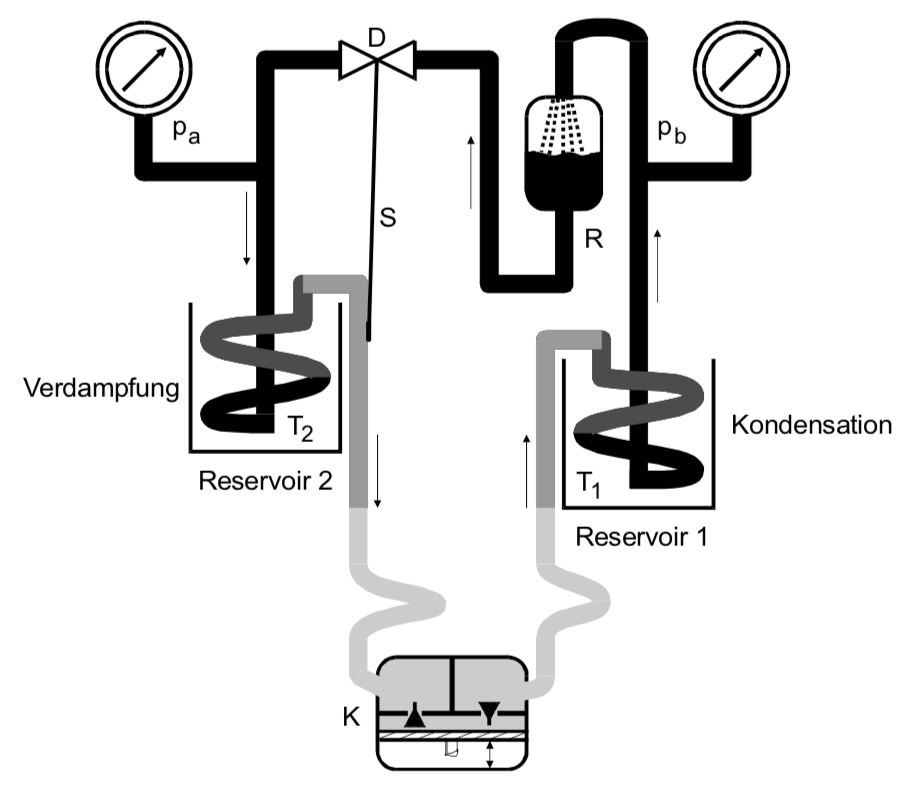
\includegraphics[width=10cm, height=10cm]{build/1.png}
    \caption{Schematischer Aufbau einer Wärmepumpe. Der Druck $p_b$ und die Temperatur
    $T_1$ beziehen sich auf das Reservoir $\num{1}$. Der Druck $p_a$ und die Temperatur
    $T_2$ beziehen sich auf das Reservoir $\num{2}$. $p_b$ und $T_1$ sind jeweils
    größer als die anderen Werte.} %Kann man das hier schon sagen? Das ist doch eher etwas, dass sich aus den Ergebnissen ergibt.
    \label{fig:aufbau1}
\end{figure}

\subsection{Bestimmung der Güteziffer}
Aus dem Quotienten aus $\Delta T_1$ und $\Delta t$ ergibt sich die pro Zeiteinheit 
gewonnene Wärmemenge zu
\begin{equation*}
    \frac{\Delta Q_1}{\Delta t} = (m_1 c_w + m_k c_k)\frac{\Delta T_1}{\Delta t}.
    \label{eqn:Q1}
\end{equation*}
$m_1 c_w$ ist dabei die Wärmekapazität des Wassers in Reservoir $\num{1}$. $m_k c_k$ ist die 
Wärmekapazität der Kupferschlange und des Eimers. Für die Güteziffer ergibt sich dann 
mit $N$ als die vom Wattmeter angezeigte und über das Zeitintervall $\Delta t$ 
gemittelte Leistungsaufnahme des Kompressors:
\begin{equation}
    \nu = \frac{\Delta Q_1}{\Delta t \cdot N} = \frac{(m_1 c_\text{w} + m_\text{k} c_\text{k})}{N} \frac{\Delta T_1}{\Delta t}.
    \label{eqn:güteziffer}
\end{equation}

\subsection{Bestimmung des Massendurchsatzes}
Für $Q_2$ lässt sich die Gleichung \ref{eqn:Q1} analog anwenden:
\begin{equation*}
    \nu = \frac{\Delta Q_2}{\Delta t \cdot N} = \frac{(m_2 c_\text{w} + m_\text{k} c_\text{k})}{N} \frac{\Delta T_2}{\Delta t}.
\end{equation*}
Für die Wärmeentnahme durch Verdampfung des Transportmediums
wird pro Massen- und Zeiteinheit die Verdampfungswärme $L$ 
verbraucht:
\begin{equation*}
    \frac{\Delta Q_2}{\Delta t} = L \frac{\Delta m}{\Delta t}.
\end{equation*}
Der Massendurchsatz wird also durch
\begin{equation}
    \frac{\Delta m}{\Delta t} = \frac{\Delta Q_2}{\Delta t \cdot L} = \frac{(m_2 c_w + m_k c_k)}{L} \frac{\Delta T}{\Delta t} %\text ergänzen
    \label{eqn:massendurchsatz}
\end{equation}
bestimmt.

\subsection{Bestimmung der mechanischen Kompressorleistung}
Die mechanische Kompressorleistung $N_{mech}$ ergibt sich zu
\begin{equation}
    N_{mech} = \frac{1}{\kappa - 1} \left(p_b \sqrt[\mathlarger{\mathlarger{\kappa}}]{\frac{p_a}{p_b}} - p_a\right)\frac{1}{\rho}\frac{\Delta m}{\Delta t}. %Müsste es hier nicht rho sein und nicht rho_0?
    \label{eqn:nmech}
\end{equation}
Dabei ist $\kappa$ das Verhältnis der Molwärmen $C_P$ und $C_V$. $\rho$ ist die Dichte
des Transportmediums im gasförmigen Zustand. Diese wird bestimmt durch
\begin{equation}
    \rho = \frac{p_a}{p_0} \frac{T_0}{T_2} \rho_0.
    \label{eqn:dichte}
\end{equation}
Die Normalbedingungen lauten $p_0 = \SI{e5}{\pascal}$ und $T_0 = \SI{273.15}{\kelvin}$.
